%===================================================================================
% JORNADA CIENTÍFICA ESTUDIANTIL - MATCOM, UH
%===================================================================================
% Esta plantilla ha sido diseñada para ser usada en los artículos de la
% Jornada Científica Estudiantil, MatCom.
%
% Por favor, siga las instrucciones de esta plantilla y rellene en las secciones
% correspondientes.
%
% NOTA: Necesitará el archivo 'jcematcom.sty' en la misma carpeta donde esté este
%       archivo para poder utilizar esta plantilla.
%===================================================================================



%===================================================================================
% PREÁMBULO
%-----------------------------------------------------------------------------------
\documentclass[a4paper,10pt,twocolumn]{article}

%===================================================================================
% Paquetes
%-----------------------------------------------------------------------------------
\usepackage{amsmath}
\usepackage{amsfonts}
\usepackage{amssymb}
\usepackage{jcematcom}
\usepackage{multicol}
\usepackage{float}
\usepackage{graphicx}
\usepackage[utf8]{inputenc}
\usepackage{listings}
\usepackage[pdftex]{hyperref}
%-----------------------------------------------------------------------------------
% Configuración
%-----------------------------------------------------------------------------------
\hypersetup{colorlinks,%
	citecolor=black,%
	filecolor=black,%
	linkcolor=black,%
	urlcolor=blue}
\graphicspath{{./res/}}

%===================================================================================



%===================================================================================
% Presentación
%-----------------------------------------------------------------------------------
% Título
%-----------------------------------------------------------------------------------
\title{Proyecto Modelos Matemáticos Aplicados \\
	Aritmética de punto flotante \\
	con cualquier precisión y cualquier base}

%-----------------------------------------------------------------------------------
% Autores
%-----------------------------------------------------------------------------------
\author{\\ Reserved \\}
%-----------------------------------------------------------------------------------
% Tutores
%-----------------------------------------------------------------------------------
\tutors{Reserved, \emph{UH}}

%-----------------------------------------------------------------------------------
% Headings
%-----------------------------------------------------------------------------------


%-----------------------------------------------------------------------------------

%===================================================================================



%===================================================================================
% DOCUMENTO
%-----------------------------------------------------------------------------------
\begin{document}
	
	%-----------------------------------------------------------------------------------
	% NO BORRAR ESTA LINEA!
	%-----------------------------------------------------------------------------------
	\twocolumn[
	%-----------------------------------------------------------------------------------
	
	\maketitle
	
	%===================================================================================
	% Resumen y Abstract
	%-----------------------------------------------------------------------------------
	\selectlanguage{spanish} % Para producir el documento en español
	
	%-----------------------------------------------------------------------------------
	% Resumen en Español
	%-----------------------------------------------------------------------------------
	\begin{abstract}
		
		El objetivo de este trabajo es poder usar en \textbf{Common Lisp} y/o \textbf{Python} una aritmética de punto flotante con precisión variable y en la que se puedan realizar operaciones \textbf{en cualquier base}. \\
		
		Por ejemplo, debe ser posible realizar operaciones con números que tengan una mantisa de tamaño 4 y estén representados en base 10, o con números que tengan una mantisa de tamaño 20 y estén representados en base 2.\\
		
		Las operaciones deben ser compatibles con el estándar \textbf{IEEE 754}. Eso quiere decir que deben estar representados los infinitos, el NaN y los modos de redondeo. No interesan números subnormales. \\
		
		Para el proyecto interesa poder realizar correctamente las operaciones aritméticas y evaluar las funciones elementales. La velocidad de ejecución no es importante.\\
		
	\end{abstract}
	
	%-----------------------------------------------------------------------------------
	% English Abstract
	%-----------------------------------------------------------------------------------
	\vspace{0.5cm}
	
	\begin{enabstract}
		
		The task of this work is to be able to use in \textbf{Common Lisp} and/or \textbf{Python} a floating point arithmetic with variable precision and in which operations can be carried out \textbf{in any base}. \\
		
		For example, it must be possible to perform operations on numbers that have a mantissa of size 4 and are represented in base 10, or with numbers that have a mantissa of size 20 and are represented in base 2.\\
		
		The operations must be compatible with the \textbf{IEEE 754} standard. That means that infinities, NaN, and rounding modes must be represented. Subnormal numbers are not of interest.\\
		
		The project is interested in being able to perform arithmetic operations correctly and evaluate elementary functions. The execution speed is not important.\\
		
	\end{enabstract}
	
	%-----------------------------------------------------------------------------------
	% Palabras clave
	%-----------------------------------------------------------------------------------
	\begin{keywords}
		\\	\textbf{Aritmética de punto Flotante},\\
		\textbf{Sistema Numérico Posicional},\\
		\textbf{Estándar IEEE 754}\\
		\textbf{Redondeo},\\
		\textbf{Errores}.
	\end{keywords}
	
	%-----------------------------------------------------------------------------------
	% Temas
	%-----------------------------------------------------------------------------------
	
	
	
	%-----------------------------------------------------------------------------------
	% NO BORRAR ESTAS LINEAS!
	%-----------------------------------------------------------------------------------
	\vspace{7cm}
	]
	\pagebreak
	%-----------------------------------------------------------------------------------
	
	
	%===================================================================================
	
	%===================================================================================
	% Introducción
	%-----------------------------------------------------------------------------------
	\section{Introducción}\label{sec:intro}
	%-----------------------------------------------------------------------------------
	Iniciamos introduciendo el concepto de \textbf{punto flotante} (floating point) el cual es una forma de notación científica basada en el sistema numérico posicional con la cual pueden representarse números reales extremadamente grandes o pequeños de una manera eficiente en un espacio discreto como en los computadores. Con estas representaciones también se pueden realizar operaciones aritméticas con gran eficacia, precisión y sin duda representan una ventaja sobre los sistemas de punto fijo.\\
	
	
	\subsection{Sistema Numérico Posicional}
	
	La notación posicional es un sistema de numeración en el cual cada dígito posee un valor que depende de su posición relativa, la cual está determinada por la base o \textbf{radix}, que es el número de dígitos necesarios para escribir cualquier número. Con la notación posicional, los cálculos aritméticos son mucho más simples que con cualquier sistema numérico anterior.\\
	
	Por ejemplo el más común es el \textbf{sistema decimal} en el cual se necesitan solo 10 dígitos (0, 1, 2, 3, 4, 5, 6, 7, 8, 9) diferentes para poder escribir cualquier valor numérico entero por muy grande o pequeño que sea. Sin embargo, el sistema numérico binario (radix 2) se usa en casi todas las computadoras y dispositivos electrónicos porque es más fácil de implementar de manera eficiente en los circuitos electrónicos. \\
	
	
	Un número en esta notación es representado en lo que se conoce como forma de Horner:
	\begin{equation}
		\sum_{i=-\infty}^{+\infty} a_i b^i
	\end{equation}
	Donde $a_i$ representa los dígitos del número representado en punto flotante, $b$ es la base en la cual vamos a trabajar e $i$ serían las posiciones del número representado en la precisión dada.\\   
	
	La posición de cada dígito depende de donde se emplace la coma en el número, siendo el dígito que la precede la posición o exponente $i=0$ y el que la antecede $i=-1$.
	
	Por ejemplo el n\'umero 102.02 en base 10
	\begin{equation}
		1*10^2 + 0*10^1 + 2*10^0 + 0 * 10 ^{-1} + 2 * 10 ^{-2} = 102,02
	\end{equation}
	
	El ejemplo anterior parece obvio pero si analizamos uno en radix 2:\\
	
	Sea el n\'umero: $10101 = 21$ en base 10\\
	
	Si emplazamos la coma de esta forma $101.01$ tendríamos el número $5,25$ en base 10 y si la emplazáramos de la siguiente manera $10.101$ tendríamos el número $2.625$ en base 10. La respuesta está en su desarrollo de Horner. Números con exponente negativo en base 2 son de la forma $1/2+ 1/4 +1/8$ por lo que se hace evidente que no será posible representar el n\'umero decimal $1/10=0.1$ el cual es un n\'umero periódico en radix 2 = $0.001001100110011001100..$ de la misma forma que $1/3$ no es representable en base 10. De hecho, el n\'umero $0.1$ solo será representable en bases potencia de 10.
	
	
	Existen infinitas bases, no solo la decimal, y a medida que se incrementa el tamaño de las bases deben agregarse nuevos símbolos (grafemas) a la representación como se aprecia en el ejemplo siguiente donde en el sistema hexadecimal el número \textbf{15} del sistema decimal es representado por la letra \textbf{F} :
	\begin{center}
		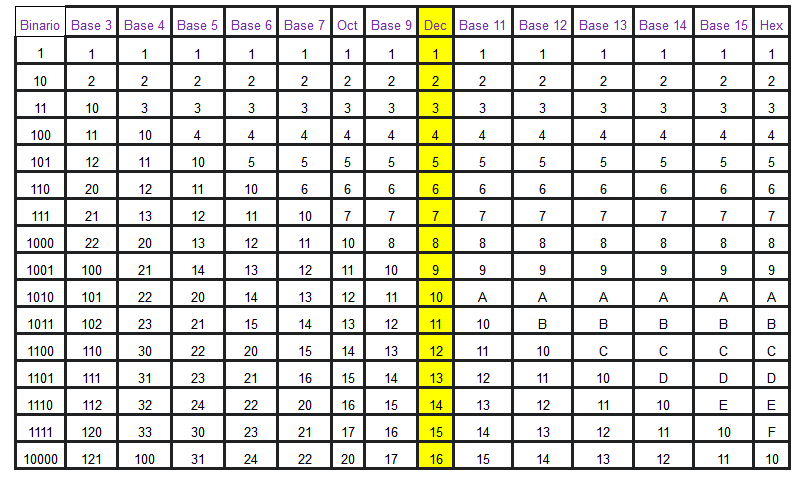
\includegraphics[scale=0.4]{tabla.png}
	\end{center}
	
	En nuestra biblioteca hemos implementado un alfabeto que opera desde el radix 2 hasta el radix 36. Si se desea agregar mayor tamaño a las bases proporcionadas debe agregarse un nuevo grafema al alfabeto predeterminado. \\       
	
	\subsection{IEEE 754}
	
	El estándar para la representación en coma flotante en hardware es el \textbf{IEEE 754} establecido en 1985 con revisiones en 2008, el cual aborda y mejora muchos de los problemas encontrados en las diversas implementaciones de representaciones de punto flotante como: \\
	\begin{itemize}
		\item[•] \textbf{Operaciones aritméticas}\\
		\item[•] \textbf{Formatos aritméticos:}
		conjuntos de datos de punto flotante binarios y decimales, que consisten en números finitos, incluidos los números subnormales, infinitos y valores especiales no numéricos (NaN). \\
		\item[•] \textbf{Reglas de redondeo:}  propiedades que deben satisfacerse al redondear los números durante las operaciones aritméticas y las conversiones.
		\item[•] \textbf{Formatos de intercambio:}  codificaciones (cadenas de bits) que se pueden utilizar para intercambiar datos de coma flotante de forma eficiente y compacta.
	\end{itemize}      
	
	Los formatos aritméticos pueden representar números finitos los cuales pueden ser de base $(b)$ 2 (binario) o de base 10 (decimal).
	
	Su precisión depende de la base y el número de dígitos de la misma en la mantisa.\\
	
	Los números de puntos flotantes de este estándar están definidos un signo, una base, un exponente y una mantisa o significando y se pueden expresar de esta forma:
	
	\begin{equation}
		v = (-1)^{s} \times m \times b^{e}
	\end{equation}
	
	Muchas representaciones de punto flotante en radix 2 tienen un \textbf{bit oculto} implícito en la mantisa. Este es un bit que está presente virtualmente en la mantisa, pero no es almacenado en memoria porque su valor es siempre 1 si el número está \textbf{normalizado} (no empieza con ceros en su representación), con lo que se consigue ganar un bit extra de precisión.\\
	
	Los números de punto flotante generalmente se normalizan debido a que, si tenemos un número no normalizado o denormal, entonces en el principio de su mantisa contiene un 0, lo cual significa que se puede restar 1 del exponente de otro número de punto flotante y obtener el mismo valor que este. Los números denormales contienen menos precisión de la que normalmente puede contener la representación. Por esto dos números de punto flotante normalizados distintos no pueden tener el mismo valor. \\
	
	
	
	
	El \textbf{Estándar IEEE 754} proporciona muchos formatos estrechamente relacionados, que difieren solo en algunos detalles. Algunos de estos formatos se denominan formatos básicos, otros formatos de precisión extendida. Los dos más conocidos son: \\
	\begin{itemize}
		\item[•] \textbf{Precisión simple:} Este es un formato binario que ocupa \textbf{32 bits (4 bytes)}, su mantisa tiene una precisión de \textbf{24 bits}, alrededor de 7 dígitos decimales. Cualquier número entero con valor absoluto menor de $2^{24}$ puede representarse en este formato. Como tal la mantisa solo tiene \textbf{23 bits} debido a que el primero se toma para representar el \textbf{bit oculto}.
		\begin{center}
			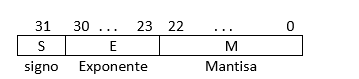
\includegraphics[scale=0.8]{representacion.png}
		\end{center}
		\item[•] \textbf{Precisión doble:} Este es un formato binario que ocupa \textbf{64 bits (8 bytes)}, su mantisa tiene una precisión de \textbf{53 bits}, alrededor de 16 dígitos decimales. Pueden representarse cualquier entero con valor absoluto menor que $2^{53}$  
		\begin{center}
			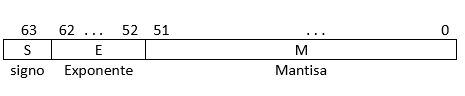
\includegraphics[scale=0.5]{representacion2.png}
		\end{center}
		
	\end{itemize}
	
	
	En nuestra biblioteca se puede trabajar con cualquier precisión del \textbf{Estándar IEEE 754} incluso con algunas que no están incluidas en este. Dada la naturaleza multibase de nuestra biblioteca no es posible tener un dígito oculto pues este  no necesariamente tiene que ser 1 para $radix > 2$\\  
	
	
	
	
	
	
	
	\subsection{Redondeo}
	
	Todos los números expresados en representación de puntos flotantes son números racionales con una expansión final en la base correspondiente, que puede ser infinita como el número $\frac{1}{3}$ en base decimal. Por esto existen números que no se pueden representar exactamente como los irracionales o algunos números que parecen cortos y exactos para una base en específico y pueden ser un dolor de cabeza en otras, como el número 0.1 representable en base decimal pero no en binario (tendría una secuencia infinita $"1100"$) por lo tanto deben aproximarse. También el número de bits de precisión limita el conjunto de números racionales que se pueden representar con exactitud, por esto a mayor precisión mejor estarán representados los números. \\
	
	Estos números no representables requieren una conversión antes de poder usarse. Esta conversión es debido a que para representarlos se necesita más dígitos que bits contenidos en la mantisa, igual sucede a veces al obtener un resultado exacto en una operación de punto flotante. Si el número puede representarse exactamente en el formato de punto flotante su conversión es exacta y si no hay una representación exacta, la conversión requiere elegir qué número de punto flotante usar para representar el valor original. La representación elegida tendrá un valor diferente al original, a este valor ajustado se le denomina \textbf{valor redondeado}.\\
	
	Para solucionar este problema \textbf{IEEE 754} requiere redondear el valor y para esto existen diferentes tipos de redondeos de los cuales implementamos los dos primeros: \\
	\begin{itemize}
		\item[•] \textbf{Redondeo al número par más cercano:} Como tal este es el modo predeterminado del estándar y es el más común, en este se redondea al dígito par más cercano en la posición requerida. \\
		\item[•] \textbf{Redondeo hacia cero:} se redondea lo más cercano al cero posible, también es considerado \textbf{truncamiento}
		\item[•]\textbf{Redondeo alejado de cero:} se redondea lo más alejado al cero posible, es más utilizado para puntos flotantes con base decimal.\\
		\item[•] \textbf{Redondeo hacia el $+\infty$:} se redondea hacia el "techo" o el infinito positivo, por lo tanto los números negativos se redondean hacia cero.\\
		\item[•]\textbf{Redondeo hacia el $-\infty$:} se redondea hacia el $-\infty$ o "piso" por lo tanto los resultados negativos se redondean alejándose de cero.
		
	\end{itemize}
	
	Dado lo antes mencionado sobre representabilidad y espacio limitado se hace necesario el Análisis del Error, lo cual es fundamental en la estimación de la precisión y su confiabilidad. Para caracterizar la precisión de una aproximación se utiliza el \textbf{error absoluto} y el \textbf{error relativo}.\\
	
	\begin{itemize}
		\item[•] \textbf{Error absoluto:} se define como la diferencia positiva entre el valor real $\bar{x}$ de una determinada magnitud y el valor estimado $x_i$ : $\Delta x =|\bar{x} - x_i|$
		
		\item[•] \textbf{Error relativo:} se define como el cociente del error absoluto y el valor real, $\bar{x}$ de la magnitud, es decir el error absoluto por unidad de magnitud o por ciento de error: $\delta x = \frac{\Delta x}{x} = \frac{|\bar{x} - x_i|}{\bar{x}}$. A veces el error relativo se calcula como por ciento multiplicando por 100 el valor numérico del error.\\
	\end{itemize}
	
	Estos tienen una estrecha relación con la precisión debido a que las cotas del error relativo dependen directamente de este. A mayor precisión, mayor será la precisión relativa alcanzable en la computadora, pues las cotas del error relativo serán menores. A la menor de las cotas superiores del error relativo se le denomina épsilon de la máquina (machine epsilon o $\epsilon -$ mach) la cual es la magnitud más útil asociada a un sistema de numeración en representación flotante, debido a que es el menor valor de una determinada máquina que cumple: $1.0 + \epsilon-mach > 1.0$. Es una consecuencia de la precisión finita de la aritmética en punto flotante.\\
	
	Si expresamos lo antes dicho en lenguaje matemático tendremos una forma de medir el error y corroborar las representaciones:
	En una aritmética con truncamiento:
	$$
	\mathrm{E}_{\text {mach }}=B^{1-P}
	$$
	En una aritmética con redondeo:
	$$
	\mathrm{E}_{\text {mach }}=\frac{1}{2} B^{1-P}
	$$
	Luego, como enunciábamos anteriormente:
	$$
	\left|\frac{\mathrm{fl}(x)-x}{x}\right| \leq \mathrm{E}_{\text {mach }} .
	$$
	
	%===================================================================================
	
	
	
	%===================================================================================
	% Desarrollo
	%-----------------------------------------------------------------------------------
	\section{Desarrollo}\label{sec:dev}
	%-----------------------------------------------------------------------------------
	
	\subsection*{Bibliotecas}
	
	Para solucionar el problema que planteamos al principio de este proyecto investigamos acerca de varias bibliotecas en las cuáles se pueden realizar operaciones de aritmética flotante: \\
	
	\begin{itemize}
		\item[•] \textbf{GMP}: \textbf{GNU Multiple Precision Arithmetic Library (GMP)} es una biblioteca libre para cálculos con aritmética de precisión múltiple  \textbf{GMP} desarrollado por \textbf{GNU Projects}, que incluye aritmética integral, racional y de punto flotante en cualquier base. Contiene muchos bindings como \textbf{General Multiprecision Python (GMPY)} el cual es un módulo de extensión de \textbf{Pyhton} y \textbf{GNU Multi-Precision Routines for SBCL} para \textbf{Common Lisp}. 
		
		\item 
		\textbf{SoftFloat:}
		Berkeley SoftFloat es una implementación de software gratuita y de alta calidad de punto flotante binario que cumple con el estándar IEEE para aritmética de punto flotante. SoftFloat es completamente fiel al estándar IEEE y, al mismo tiempo, es relativamente rápido. 
		
		Estas bibliotecas no permiten cambio de base y no es factible implementar uno pues no se tienen en cuenta los errores de representabilidad en una base y los errores que propagaría al realizar las operaciones.
	\end{itemize}
	
	
	\subsection{Nuestra biblioteca}
	
	Nuestra biblioteca provee las operaciones aritmético-lógicas básicas requeridas en el IEEE 754, representabilidad multibase hacia las aritméticas y desde las mismas, y dos modos de redondeo.\\
	
	Está desarrollada en Python 3.9 y consta de una clase llamada $Extended754$ \\
	\begin{figure}[H]
		\centering
		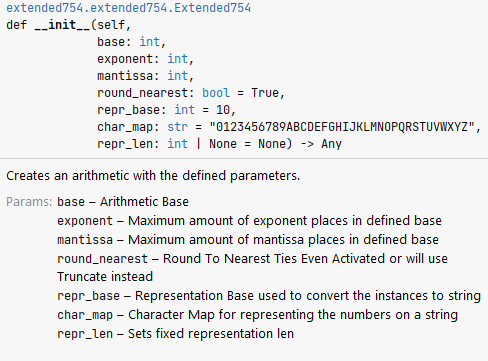
\includegraphics[width=1.1\linewidth]{res/extendedclass}
		\caption{Clase Extended754 con la cual se pueden crear instancias de aritméticas}
	\end{figure}
	
	
	que recibe la base de la aritmética, el tamaño de su exponente y el tamaño de su mantisa. Opcionalmente recibe si tendrá redondeo por truncamiento ya que el redondeo al más cercano es el por defecto como en el estándar IEEE 754.\\
	
	Además un mapa de caracteres opcional también que por defecto tiene 36 chars "0-9,A-Z" y en qué base preferiría visualizar los números la cual por defecto es 10.
	
	Con las aritméticas creadas se pueden instanciar clases \texttt{efloat}  recibiendo un string o un número y un entero que indica su base de entrada, como se observa en el siguiente y famoso ejemplo.

	\onecolumn
	\subsection{Ejemplos de Uso}
	A continuación mostraremos algunos ejemplos a modo de tutorial, a la derecha de cada l\'inea se muestra su evaluación en el debugger:
	\begin{figure}[H]
		\centering
		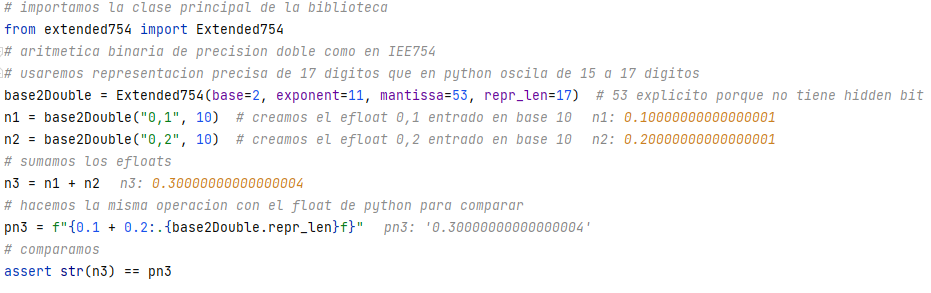
\includegraphics[width=0.9\linewidth]{res/screenshot001}
		\caption{Ejemplo famoso de la suma de 0.1 + 0.2 implementado en una aritmética 754 doble de base 2}
	\end{figure}

\begin{figure}[H]
	\centering
	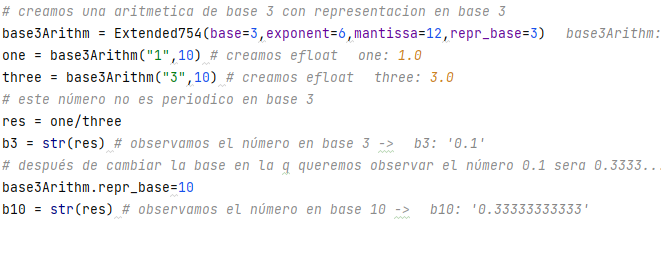
\includegraphics[width=0.9 \linewidth]{res/base3}
	\caption{Ejemplo de división en una aritmética en base 3}
	\label{fig:base3}
\end{figure}

\begin{figure}[H]
	\centering
	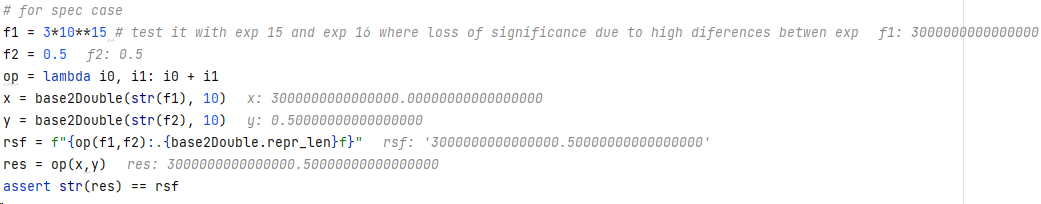
\includegraphics[width=0.9 \linewidth]{res/sigloss0}
	\caption{Ejemplo sin pérdida de significancia número con exponente 15}
	\label{fig:sigloss0}
\end{figure}

\begin{figure}[H]
	\centering
	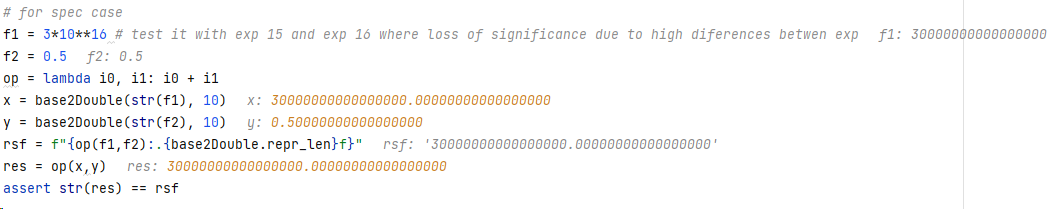
\includegraphics[width=0.9\linewidth]{res/sigloss1}
	\caption{Ejemplo con pérdida de significancia número con exponente 16}
	\label{fig:sigloss1}
\end{figure}




	\twocolumn
	\subsection{Detalles de Implementación}
	
	Como mencionábamos anteriormente nuestras aritméticas no poseen hidden bit pues son multibase, por lo que hay que declarar explícitamente la cantidad de elementos de la mantisa.
	
	Nuestras aritméticas poseen redondeo al par más cercano(por defecto en nuestra lib y en el IEEE 754) y redondeo por truncamiento (otro de los más utilizados).\\
	
	Nuestra clase \texttt{efloat}  consiste en: \\
	
	Una \textbf{mantisa} normalizada que es un arreglo de dígitos de la base de la aritmética y de tamaño igual al especificado en la misma. Una ventaja de este acercamiento es que no sufriremos pérdida de precisión al no utilizar por ejemplo cadenas de bits en la que habría efecto de \textbf{wobbling precision} (efecto de pérdida de precisión al representar números de $bases > 2$ en mantisas binarias normalizadas como por ejemplo en aritméticas hexadecimales donde cada unidad es un nibble y la mantisa 0001 0000 0000 ... esta normalizada sin embargo tiene 3 bits de pérdida de precisión).\\
	
	Un entero \textbf{exponente} que puede aceptar valores como máximo valor absoluto del bias de la aritmética (es un número igual a $b^{len(exp)-1}-1$) que se utiliza en binario para evitar utilizar complemento a dos para los distintos signos del exponente por lo que a cada uno se le añade o resta este bias. Un número mayor que este en valor absoluto constituye un desbordamiento y por tanto un NaN o infinito.\\
	
	Un entero \textbf{signo} que puede tomar 1 o -1 en dependencia del signo del número, lo cual resulta más cómodo que el 0 para algunas operaciones internas como transferencia de signo.\\
	
	
	Estos "efloat" tienen implementadas las siguientes operaciones que se definen a continuación:
	
	
	\subsubsection{Operaciones de la Aritmética de Punto Flotante}
	
	Para la aritmética de punto flotante existen operaciones aritméticas y lógicas que no pueden faltar y nuestra biblioteca las implementa de esta forma: \\ 
	\begin{itemize}
		\item[•] \textbf{Adición y Sustracción}:  
		\begin{align}
			X_1 + X_2 &= X_3 \\
			(m_1 \times b^{e_1}) +/- (m_2 \times b^{e_2})  &= X_3 
		\end{align}
		\textbf{Pasos a seguir:}\\
		\begin{itemize}
			\item[1-] $X_1$ y $X_2$ solo pueden sumarse o restarse si sus exponentes son iguales ($e_1 = e_2$). \\
			\item[2-] Suponemos que $X_1$ tiene el mayor valor absoluto de los 2 números, sino intercambiamos los valores de $X_1$ y $X_2$ : $Abs(X_1)> Abs(X_2)$.\\
			\item[3-] El valor inicial del exponente debe ser el mayor de los 2 exponentes, como sabemos que el exponente de $X_1$ será mayor, entonces $e_3 = e_1$.\\
			\item[4-] Se calcula la diferencia entre los exponentes $e_1 - e_2$.\\
			\item[5-] Se desplaza a la izquierda el punto flotante de la mantisa $m_2$ por la diferencia de los exponentes. Por lo tanto los exponentes $e_1$ y $e_2$ serán iguales.\\
			\item[6-] Se calcula la suma/diferencia de las mantisas según el bit de signo $s_1$ y $s_2$. Si los signos de $x_1$ y $x_2$ son iguales $(s_1 = s_2)$, entonces se suman las mantisas $m_1 + m_2$. Si los signos de $x_1$ y $x_2$ no son iguales $(s_1 \neq s_2)$ entonces se restan las mantisas.\\ 
			\item[7-] Se normaliza la mantisa resultante $m_3$ si es necesario y $e_3$ se ajusta de acuerdo con la normalización de la mantisa.
		\end{itemize}
		
		
		\item[•] \textbf{Multiplicación}:   
		\begin{align}
			X_1 * X_2 &= X_3\\
			(-1)^{s_1} ( m_1 \times b^{e_1}) * (-1)^{s_2} ( m_2 \times b^{e_2}) &= X_3
		\end{align}   
		$s_1 , s_2$: Son el bit del signo de los números de punto flotante $X_1$ y $X_2$ respectivamente. \\
		$e_1 , e_2$: Son los bits del exponente de  $X_1$ y $X_2$ respectivamente.\\
		$m_1 , m_2$: Son los bits de la mantisa de  $X_1$ y $X_2$ respectivamente.\\
		
		\textbf{Pasos a seguir:}
		\begin{itemize}
			\item[1-] Comprobar si uno o ambos factores son \textbf{0} o \textbf{infinito}, si esto se cumple entonces  el resultado será 0 o infinito. \\
			\item[2-] Se calcula el bit del signo resultante aplicando $s_1$ xor $s_2$. \\
			\item[3-] Se multiplican las mantisas $m_1$ y $m_2$ y se coloca el resultado en la mantisa resultante. Se aplicarán operaciones de redondeo o truncamiento según la precisión en donde se trabaje. \\
			\item[4-] Los bits de los exponentes se suman ($e_1 + e_2$) luego se agrega a los bits del exponente resultante. \\
			\item[5-] Se normaliza el número ya sea desplazando el punto (coma) a la derecha e incrementando el exponente o desplazándolo a la izquierda y disminuyendo el exponente. \\
		\end{itemize}
		\item[•]\textbf{División}: La división en \textbf{IEEE 754} se realiza dividiendo las mantisas de los dividendos y restando sus exponentes:\\
		\begin{align}
			X_1 / X_2 &= X_3\\
			(-1)^{s_1} ( m_1 \times b^{e_1}) / (-1)^{s_2} ( m_2 \times b^{e_2}) &= X_3  \\
			(-1)^{s_3} (m_1 / m_2) b^{e_1-e_2} &= X_3
		\end{align} 
		\textbf{Pasos a seguir:}
		\begin{itemize}
			\item[1-] Si el divisor $X_2 = 0$ ,  el resultado es \textbf{infinito}, si tanto $X_1$ como $X_2$ son cero, el resultado es \textbf{NAN}.(Aunque esto no garantiza que no haya desbordamiento) \\
			\item[2-] Bit del signo $s_3 = s_1$ xor $s_2$. \\
			\item[3-] $m_3 = m_1 / m_2$. \\
			\item[4-] $e_3 = e_1 - e_2$
			\item[5-] Se normaliza si es requerido como explicamos en la multiplicación.\\
		\end{itemize}
   

   
 La operación de división puede expresarse como $ab^{-1}$ donde $a$ es el dividendo y $b$ es el divisor. 
 \\\\
 El recíproco de la mantisa es la parte más crucial del cálculo, ya que es el paso más lento y puede introducir errores de redondeo. Este cálculo se realiza mediante los siguientes métodos \cite{Handbook} \cite{Divpaper}:
 \begin{itemize}
 \item[•] \textbf{Recurrencia de dígitos}: Los algoritmos de recurrencia de dígitos, como la familia de algoritmos SRT que llevan el nombre de Sweeney, Robertson y Tocher, generalizan el algoritmo de papel y lápiz aprendido en la escuela, su latencia es mas largas\\
 
 \item[•]  \textbf{Iteraci\'on funcional}: Se pueden utilizar algoritmos como \textbf{Newton-Raphson} o\textbf{ Goldschmidt}. Estos algoritmos son rápidos, escalables y tienen alta precisión.\\
  
  \item[•] \textbf{Aritm\'etica de radixes m\'as altos}:  este método es rápido pero muy complicado\\
 \end{itemize}
    
 El algoritmo de \textbf{Newton-Raphson} necesita un valor inicial $x_0$ el cual denota la suposici\'on inicial de la ra\'iz y puede converger r\'apidamente cuando la suposici\'on inicial es bastante cercana a la ra\'iz deseada.  \\

Su ecuaci\'on de recurrencia es la siguiente:
$$
x_{n+1}=x_{n}-\frac{f\left(x_{n}\right)}{f^{\prime}\left(x_{n}\right)}
$$
donde $f'(x_0)$ es la primera derivada con respecto a x.

Necesitamos una función objetivo $f(x)$ cuya raíz sea $\frac{1}{b}$

La cual es:
$$
f(x)=\frac{1}{x}-b
$$
	
Calculamos su derivada sustituimos y transformamos:

$$
\begin{aligned}
	f^{\prime}(x) &=-\frac{1}{x^{2}} \\
	x_{n+1} &=x_{n}-\frac{\frac{1}{x_{n}}-b}{-\frac{1}{x_{n}^{2}}} \cdot \frac{-x_{n}^{2}}{-x_{n}^{2}} \\
	&=x_{n}-\left(-x_{n}+b x_{n}^{2}\right) \\
	&=2 x_{n}-b x_{n}^{2} \\
	&=x_{n} \cdot\left(2-b x_{n}\right)
\end{aligned}
$$


Lo cual solo requiere de dos multiplicaciones y una resta para poder computar la ecuación.\\

\textbf{Cálculo del valor inicial con lookup tables}:

La mantisa de n-bits está representada por : \\
\begin{equation}
1.m_1 m_2 m_3 ... m{n-1} (m_i \in {0,1}, i = 1... n)
\end{equation}

Si dividimos $M$ en dos partes $M_1$ y $M_2$: \\
\begin{align}
M_1 &= 1.m_1 m_2 m_3 ... m_m \\
M_2 &= 0. m_{m+1} m_{m+2} m_{m+3} ... m_{n-1}
\end{align}

La expansión de primer orden de Taylor $M^p$ de número $M$ entre $M_1$ y $M_1 + 2^{-m}$ se expresa como: \\
\begin{equation}
(M_1 - 2^{-m-1})^{p-1} * (M_1 + 2 ^{-m-1} + p * (M_2 - 2^{-m-1}))
\end{equation} 

la cual puede ser expresada por :
\begin{align*}
 C &\times M \\
 C &= (M_1 - 2 ^{-m-1})^{p-1} \\
 M &= M_1 + 2^{-m-1} + p \times (M_2 - 2^{-m-1})
\end{align*}

$C$ se puede leer desde una tabla de búsqueda que contiene los $2^m$ valores de $C$ para los valores especiales de $p$, donde es $-2^{0}$ para el recíproco de $M$. El tamaño requerido para la tabla de búsqueda es $2^m \times 2m$ bits. \\

La aproximación inicial del número de punto flotante $M^{-1}$ se computa con la multiplicación del término $C$ con la forma modficada de $M$, la cual se obtiene complementándolo con $M_2$ bit a bit. \\




\textbf{Nuestra aproximación del valor inicial}:

Al ser aritméticas multibase la inicialización de lookup tables sería necesaria para cada base al crearla y de forma general.
Sin embargo al ser emulada en software podemos partir de un valor inicial con errores utilizando el doble en base dos de python,
lo cual es una muy buena aproximación.

		\item \textbf{Operaciones Lógicas de Orden}:
		Las operaciones lógicas de orden siguen el siguiente formato basándonos en el orden estricto mayor:\\
		
		Un número flotante es mayor que otro si su signo es mayor, sino si su exponente es mayor, o sino si su mantisa es     mayor.\\
		Análogamente implementamos las demás operaciones de orden.\\
		A continuación, se muestra como manejamos las operaciones con símbolos especiales: \\
		Cualquier operación aritmética que implique un NaN tiene como resultado NaN.\\
		Además:
		\begin{figure}[H]
			\centering
			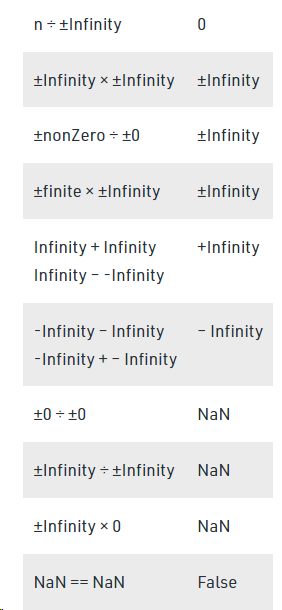
\includegraphics[width=0.7\linewidth]{res/screenshot002}
			\caption{Resultados Especiales}
			\label{}
		\end{figure}
		
	\end{itemize}
	
	
	Todas estas operaciones las realizamos a través de los big int de python los cu\'ales son rápidos, interpretando la mantisa como un número entero, operando, y re-interpretando la mantisa, normalizando y redondeando posteriormente.
	
	
	
	%-----------------------------------------------------------------------------------
	
	%-----------------------------------------------------------------------------------
	
	
	%-----------------------------------------------------------------------------------
	
	%-----------------------------------------------------------------------------------
	
	
	%===================================================================================
	
	
	
	%===================================================================================
	% Conclusiones
	%-----------------------------------------------------------------------------------
	\section{Conclusiones}\label{sec:conc}
	
	La notación de punto flotante es una compleja pero muy útil notación científica. Comprender las operaciones de punto flotante en el \textbf{Estándar IEEE 754}, sus posibles representaciones, errores entre otros requiere de un gran conocimiento matemático. Si adicionamos salir de los esquemas de poder trabajar con precisiones y bases predeterminadas (como la binaria y la decimal que son de las más usadas), se complejiza aún más. Primero que el algoritmo a realizar debe de ser lo más genérico posible debido al amplio rango de bases en las que se pueden realizar las operaciones, además poder realizar estas operaciones evitando o reduciendo lo máximo posible todos los errores intermedios y finales, lo cual conlleva ciertos conocimientos adicionales acerca de algoritmos auxiliares para su resolución. Esta biblioteca de precisión variable y con operaciones en cualquier base expande las representaciones y operaciones del \textbf{Estándar IEEE 754} en el cual se profundiza más en las representaciones en otras bases usualmente no utilizadas.
	
	%===================================================================================
	
	
	
	%===================================================================================
	
	
	
	
	%===================================================================================
	
	
	
	%===================================================================================
	% Bibliografía
	%-----------------------------------------------------------------------------------
	\begin{thebibliography}{99}
		%-----------------------------------------------------------------------------------
		\bibitem{Converter} \textbf{Sitio Recomendado} FloatConverter {https://www.h-schmidt.net/FloatConverter/IEEE754.html}
		
		\bibitem{Handbook}  \textbf{Libro Recomendado} Handbook of floating-point arithmetic { by Jean-Michel Muller, Nicolas Brisebarre, Florent de Dinechin, Claude-Pierre Jeannerod, Vincent Lefèvre, Guillaume Melquiond, Nathalie Revol, Damien Stehlé, Serg}
		
		\bibitem{Divpaper}  \textbf{Paper Recomendado} A Single/Double Precision Floating-Point Reciprocal Unit Design for Multimedia Applications
		{by Metin Mete Özbilen and Mustafa Gök	Mersin University, Engineering Faculty, Department of Computer Science, Turkey}
		
		\bibitem{GNU} GNU Manual https://www.gnu.org/software/libc/manual/html-node/Floating-Point-Concepts.html
		
		\bibitem{Tutorials} Tutorials https://www.rfwireless-world.com/Tutorials/floating-point-tutorial.html
		
		
		\bibitem{Knuth} Donald E. Knuth.(1997) {The Art of Computer Programming}.
		Section 4.2: Floating-Point Arithmetic , (1997).
		
		\bibitem{wiki} Wikipedia. URL: http://en.wikipedia.org
		Floating-point arithmetic ,
		Rounding ,
		Arbitrary-precision arithmetic, 
		Horners method, 
		Sterbenz lemma 
		
	
		
		%-----------------------------------------------------------------------------------
	\end{thebibliography}
	
	\pagebreak
	
	\section{Recomendaciones}
	
	Existe lugar para la mejora en esta biblioteca utilizando solamente las mantisas como números enteros de Python que no tienen límite de tamaño y son rápidos, controlando sus tamaños con esta fórmula:
	\texttt{ math.floor(math.log(num)/math.log(base))}. Con esto también se evitan los pasos extra de normalización.\\
	
	Durante el desarrollo de esta biblioteca nos fue muy útil el sitio Float converter \cite{Converter}:
	
	\begin{figure}[H]
		\centering
		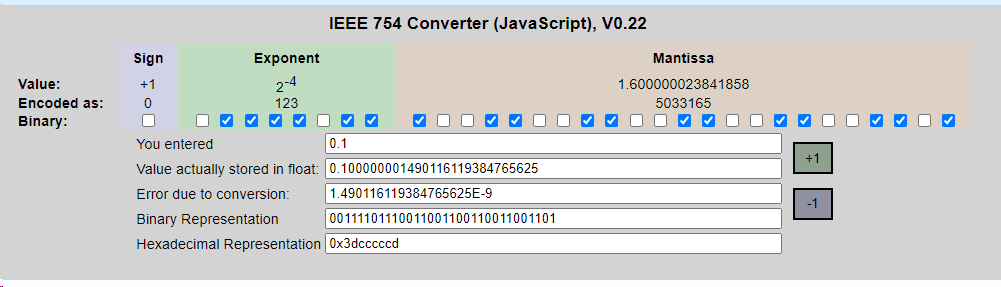
\includegraphics[width=1.1\linewidth]{res/screenshot003}
		\caption{Float converter: floats interactivos iee754}
	\end{figure}
	
	
	
	
	%-----------------------------------------------------------------------------------
	
	\label{end}
	
\end{document}

%===================================================================================
